
\chapter{Introduction}
La gestion de projet de projet couvre l’ensemble des outils, techniques et méthodes qui permettent au chef de projet et à l’équipe de projet de conduire, coordonner et harmoniser les diverses tâches exécutées dans le cadre du projet, afin qu’il satisfasse aux besoins explicites et implicites pour lesquels il a été entrepris. 
Les activités prises en charges ans le cadre d’un projet s’organisent en une suite d’étapes liées les unes aux autres. Les résultats se traduisent dans un livrable qui peut être un produit ou un service. 

\section{A propos du projet: livrable d'un service}
En application sur notre sujet, il s’agit d’un livrable qui est un service. En l’occurrence, la mise à disposition de bornes interactives sur le campus du SOLBOSCH. 
L’avant-projet est constitué de tâches qui sont dites «préparatoires» au projet. Elles vont permettre de décider notamment, s’il est opportun d’investir ou non dans le projet. 

L’élément principal de cet avant-projet est le business case ou étude d’opportunité. LE business case restera tout au long du projet, il en sera le fil conducteur puisqu’il permettra de valider que les résultats obtenus correspondent aux objectifs initiaux. 

Le business va permettre de donner un cadre au projet d’étudier la demande qui est faite, définir le périmètre souhaité, analyser les impacts qu’aura le projet à différents niveaux (organisationnel, financier, technique) mais aussi les enjeux, les bénéfices, les ressources, le délai et les risques liés au projet. 

 
\section{Etat des lieux}

\begin{comment}
Concernant notre sujet, après état des lieux de la situation actuelle sur le campus du SOLBOSCH, seulement deux ou trois panneaux situés à certaines entrées du campus affichent le plan. Le premier problème qui se pose est la localisation des panneaux, ils ne sont situés aux entrées principales du campus ce qui en réduit considérablement leur utilité et leur visibilité. Leur faible nombre est tout aussi problématique, il est très difficile voire impossible pour plusieurs étudiants de regarder le plan en même temps. Dernier problème et non des moindres, aucun panneau existant ne se trouve sur le campus même, il faut donc ressortir du campus pour avoir accès à ces panneaux et au plan. 

Étant nous-même étudiant et ayant une bonne connaissance du campus à ce jour, il nous est tous arrivé au moins une fois de se perdre dans le campus à la recherche désespéré de notre salle de cours sans aucun moyen existant pour trouver notre chemin résultant d’une arrivée après le début du cours. Lorsqu’on connaît le nombre d’étudiants, de visiteurs qui circulent sur le campus chaque année, ainsi que la taille du campus qui n’est pas négligeable, il est primordial d’apporter une solution adéquate. 

\end{comment}

Actuellement, sur le campus du Solbosh,  nous retrouvons  des panneaux  avec le plan du campus  à certaines entrées  mais pas à toutes. Nous retrouvons également des panneaux d'indication de direction à l’intérieur du campus ainsi qu’une plaque identifiant chaque entrée. 

Malheureusement, ces dispositifs sont en nombre trop restreint  pour guider convenablement les visiteurs. En outre, la vétusté  des panneaux rend ces derniers difficilement lisibles et la disposition des locaux à l’intérieur des bâtiments est parfois contre-intuitive (par exemple : l’auditoire Lameere  dont l’identifiant (UB2.252) le situe au 2ième étage, mais dont les entrées sont au rez-de-chaussée par le square  G ou par le couloir du 4ième étage).  

En résumé, il peut  être laborieux pour une personne non-habituée  au campus de s’y retrouver uniquement avec  les indications actuellement présentes. 


 
\section{Objectifs du projet}
Le projet a pour but mettre en place des bornes interactives à l’intérieur même du campus du Solbosh à différents endroits clés du campus comme par exemples les entrées principales ou bien encore devant les bâtiments importants du campus. Ils contiendront différentes informations relatives au campus telles que : 
\begin{itemize}
    \item Le plan du campus avec la localisation des auditoires, des bibliothèques, des bureaux des facultaires, des bâtiments administratifs  et des autres services proposés sur le campus (restaurants, librairies, salle de sport, associations étudiantes, etc. ) 
    \item Les horaires et le calendrier des cours, des conférences ou autres activités organisée par l'université. 
    \item Les informations personnalisées sur base du NetID ou d’un autre token d’identification 
\end{itemize}

L’objectif de ce projet est de pouvoir guider les étudiants, ou n’importe quels autres visiteurs, dans le campus su Solbosh. La borne interactive indiquerait le chemin à suivre jusqu’au bâtiment, local ou service souhaité en y entrant le numéro dudit local. 

Nous souhaitons également ajouter des fonctionnalités de personnalisation de contenu ; l’étudiant se connecterai avec son NetID (ou en scannant  le code barre de sa carte étudiant). De cette façon, l’étudiant pourrait avoir accès directement à son horaire personnalisé (Gehol), les locaux, aux valves publiées sur l’université virtuelle.  




\begin{comment}
Le projet a pour objectif de mettre en place des bornes interactives au sein même du campus SOLBOSCH, à différents endroits clés du campus comme par exemples les entrées principales ou bien encore devant les bâtiments importants du campus. Ils contiendront différentes informations relatives au campus telles que le plan du campus, les différentes salles de cours, la localisation des facultés sur le campus, ainsi que les bâtiments administratifs mais aussi la bibliothèque, les divers lieux de restaurations ou bien encore le gymnase. 

Des informations essentielles qui répondront parfaitement à l’objectif numéro un de ce projet qui est de pouvoir guider les étudiants et n’importe quels autres visiteurs dans le campus SOLBOSCH. 

La borne interactive indiquera le chemin à suivre jusqu’au local où souhaite se rendre l’utilisateur alors que celui-ci encoderait simplement le nom ou numéro du local recherché. 

Nous pouvons également ajouter une fonctionnalité de personnalisation de contenu, l’étudiant se connecte (ou scanne sa carte étudiant avec le code barre fourni au verso). De cette façon, l’étudiant pourrait avoir accès directement à son horaire personnalisé (GEHOL), les locaux, ses groupes de TP, les informations importantes publiées sur l’université virtuelle.  

Cette dualité (personnalisation via la carte étudiante et encodage simple d’un numéro ou d’un nom de local) permettrait de rendre le système accessible aux étudiants, nouveaux étudiants et visiteurs. 
\end{comment}

\section{Utilisateurs cibles}
\begin{comment}
Maintenant que l’état des lieux ainsi que la définition des objectifs du projet ont été établis, les utilisateurs cibles peuvent être déterminé. Deux catégories d’utilisateurs cibles sont ressorties.  
\subsection{Les personnes internes à l'université (étudiants, académiques, membres du personnel)}
Tout d’abord, la première catégorie d’utilisateurs cibles, sera principalement toutes les personnes qui ne sont pas familières avec le campus, c’est-à-dire les nouveaux étudiants principalement, mais aussi toutes sortes de visiteurs. D’autres utilisateurs cibles peuvent être considérés comme les étudiants qui travaillent pour l’université lors des journées portes ouvertes ainsi que les membres de l’administration à certains moments. 
\subsection{Les personnes externes à l'université (visiteurs, etc.)}
Ensuite, la seconde catégorie correspond aux visiteurs de l’ULB. Ils pourront être également concernés par la mise à disposition de bornes. En effet, l’Université organise des événements académiques, mais également culturels. 

\end{comment}

Les utilisateurs cibles seront les personnes non-familières avec le campus. Donc principalement les  nouveaux étudiants ou les visiteurs occasionnel venant assister aux évènements culturels proposé par l’université, mais aussi les étudiants Erasmus et les invités internationaux pour qui communiquer en français ne serait pas aisé. D’autres utilisateurs, plus ponctuels, peuvent être considérés : les étudiants travaillant pour l’université lors des journées portes ouvertes, ou encore le personnelle administratif de l’université ou des techniciens extérieur au campus.



\section{Objectifs SMART}
Dans le but de piloter sereinement son activité tout en ayant la garantie de déployer efficacement une stratégie visant à répondre précisément aux enjeux fixés en amont, l’utilisation de la matrice SMART permettra de fixer des objectifs concrets et s’assurer que vous pourrez les évaluer quantitativement ou qualitativement dans un laps de temps donné. 
Par la prolongation de l’état des lieux et de la définition des objectifs, quatre objectifs SMART ont été fixés: 
\begin{enumerate}
    \item « En tant que nouvel étudiant sur le campus SOLBOSCH, mon objectif est de pouvoir me rendre à ma séance d’accueil en moins de 15 minutes en empruntant un chemin simple et rapide, que je pourrais reprendre à chaque fois». (fig.\ref{smart1})
    \begin{figure} [h]
        \label{smart1} \caption{}
        \centering
        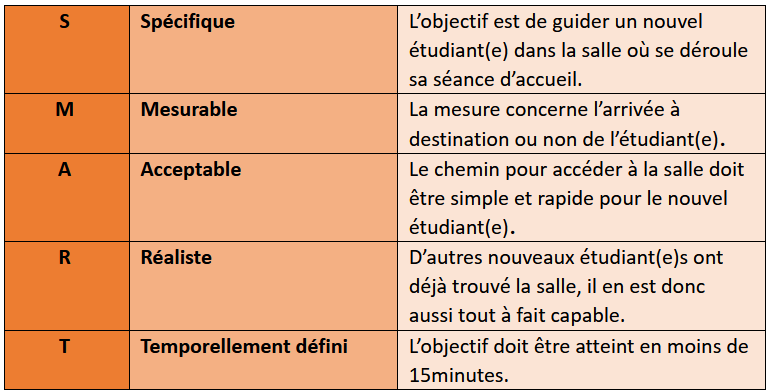
\includegraphics[width=13cm]{Pictures/smart1.png}
    \end{figure}


    \item « En tant que visiteur externe, mon objectif est de me rendre à temps au local où se déroule une conférence à laquelle je souhaite assister, en ne connaissant ni le campus, ni le bâtiment où la conférence se déroule» (fig.\ref{smart2})
    \begin{figure} [h]
        \label{smart2} \caption{}
        \centering
        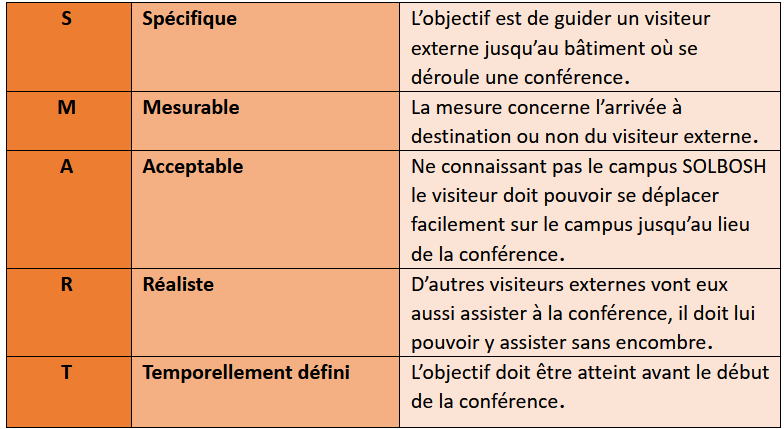
\includegraphics[width=13cm]{Pictures/smart2.png}
    \end{figure}
    \item « En tant qu’étudiant(e), mon objectif est de participer à un évènement se déroulant sur le campus SOLBOSH, plus particulièrement la Brassicole du Semeur, en ne connaissant ni la date et le lieu où se déroule l’évènement.» (fig.\ref{smart3})
    \begin{figure} [H]
        \label{smart3} \caption{}
        \centering
        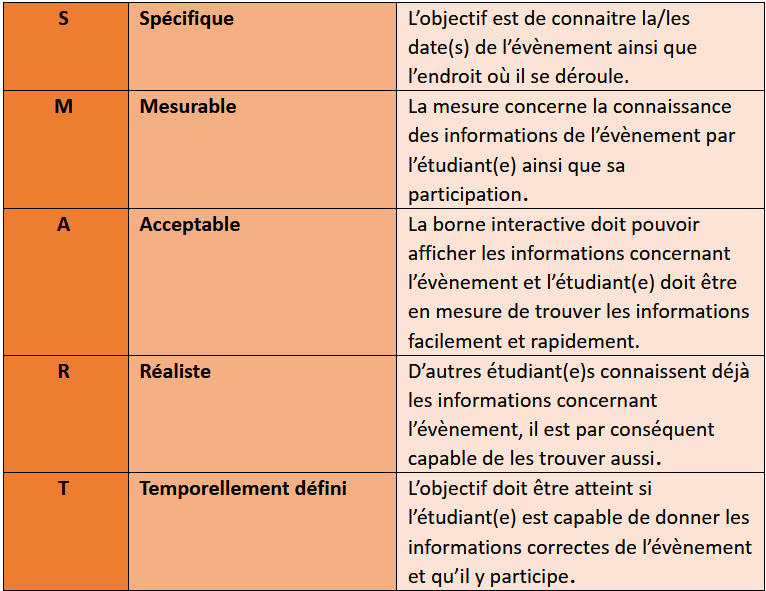
\includegraphics[width=13cm]{Pictures/smart3.png}
    \end{figure}
    \item « En tant qu’étudiant(e), mon objectif est d’aller faire du sport, plus particulièrement participer au cours de yoga organiser par l’université mais afin d’y assister j’ai besoin d’en connaitre les horaires.» (fig.\ref{smart4})
    \begin{figure} [h]
        \label{smart4} \caption{}
        \centering
        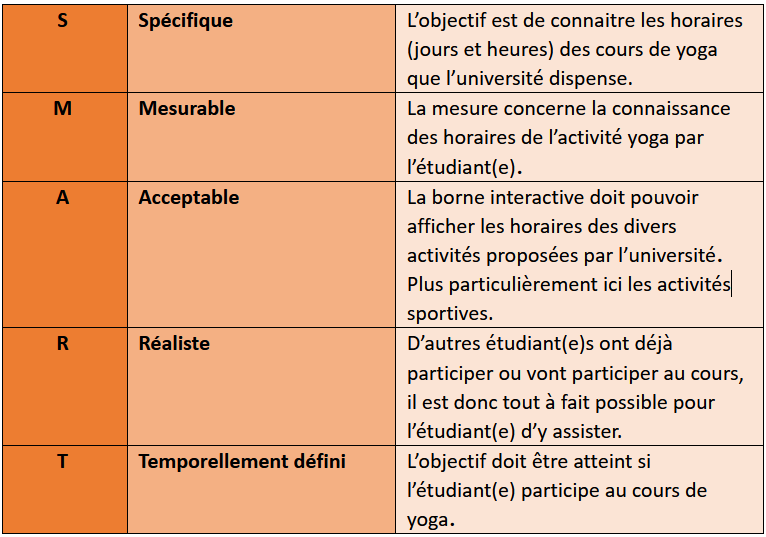
\includegraphics[width=13cm]{Pictures/smart4.png}
    \end{figure}
\end{enumerate}

\include{Tables/tb_smart}
